\documentclass[12pt]{article}
\usepackage[utf8]{inputenc}
\usepackage[english, spanish]{babel}
\usepackage{graphicx}
\usepackage{float}
\usepackage{amsmath}
\usepackage{xcolor}
\usepackage{enumitem}
\usepackage{titlesec}
\usepackage{amssymb}
\usepackage{bm}
\usepackage{booktabs}
\usepackage[round]{harvard}

\title{Método de Broyden}
\author{Leonard David Vivas Dallos \\ Tomás Escobar Rivera \\ Grupo 13}
\date{\today}

\begin{document}

\maketitle

\tableofcontents

\section{Introducción}

En el universo del análisis numérico y la optimización, el método de Broyden surge como un ingenio en términos de adaptabilidad. Un método por el cual su creador, Charles George Broyden deja una marca en la resolución de ecuaciones no lineales, y por tanto, una huella en el estudio de estos mismos. Así pues, en el presente artículo, se abordará el método de Broyden como una solución para la resolución de sistemas de ecuaciones no lineales. Se procederá a examinar tanto su motivación como su contexto histórico, seguido de una descripción acompañada de ejemplificaciones para una mayor claridad y, finalmente, un análisis detenido y detallado del mismo. Esto, con el fin de evidenciar cómo se logra llegar a un método que evade el cálculo del Jacobiano, cálculo costoso y así reduce la cantidad de operaciones aritméticas, evidenciando su utilidad y adaptabilidad a distintas situaciones.

\section{Historia}

En $1965$, Broyden presentó una categoría de métodos dirigidos a la resolución de ecuaciones simultáneas no lineales, con el propósito de mejorar el método de Newton. El autor identifica algunas limitaciones inherentes a dicho método, destacando, principalmente, que el jacobiano es difícil de computar, incluso cuando se utiliza una aproximación, y la posibilidad de divergencia. No obstante, se aprecia un aspecto favorable en la simplicidad del algoritmo y su eficiencia. ¿Qué ocurriría si pudiéramos minimizar el número de evaluaciones del jacobiano, proponer un método para actualizarlo y prevenir la divergencia? Broyden menciona el método de Newton y posteriormente introduce una variable denominada $B$, la cual representa una aproximación del jacobiano. Asimismo, emplea la variable $t$ para evitar la divergencia.

Así es como el método de Broyden, se deriva del método generalizado de Newton. Algunos argumentan que proviene del método de la secante, basándose en la reutilización del punto anterior y la similitud de notación. Se podría sostener que, debido a la reutilización del punto anterior y la notación similar, este método representa una generalización del método de la secante. En la literatura, es común encontrar afirmaciones que indican que Broyden describe una categoría de métodos secantes basados en la secante y la ecuación. No obstante, algunos, como Broyden, señalan que en su artículo sobre la mejora del método de Newton, nunca empleó la palabra \textit{secante}, además de que su método requiere condiciones iniciales que parten de un solo punto y del jacobiano, a diferencia de dicho método. Si hubiera intentado generalizar el método secante, habría dado lugar a pasos colineales en lugar de la orientación ortogonal que finalmente adoptó.

\section{Motivación}

En un cuidadoso análisis del método de Newton, Broyden nota dos desventajas de dicho método en términos de practicidad y aplicabilidad. El primero de estos radica en la dificultad en la computación de la matriz Jacobiana, ya que sin importar de la complejidad de las funciones $f_j$, la cantidad de evaluaciones de las $n^2$ derivadas parecía un poco excesiva. Más aún, en la práctica,  cuando la evaluación exacta de las derivadas parciales es complicada y se usan aproximaciones de diferencia finita a dichas derivadas parciales, como por ejemplo:

\begin{equation*}
    \frac{\partial f_j}{\partial x_k} (x^{(i)}) \approx \frac{f_j (x^{(i)} + e_k h) - f_j (x^{(i)})}{h}
\end{equation*}
donde $h$ es pequeño en valor absoluto y $e_k$ es el vector cuyo único elemento diferente de cero es $1$ en la k-ésima coordenada.

Este tipo de aproximaciones aún requieren de la realización de por lo menos $n^2$ evaluaciones funcionales escalares para realizar la aproximación del Jacobiano y por ende, no reduce la cantidad de cálculos necesarios, el cual por lo general es $O(n^3)$ para resolver el sistema lineal que contiene al Jacobiano aproximado. Así pues, el esfuerzo total necesario para una sola iteración en el método de Newton es de por lo menos, ($n^2+n$) evaluaciones funcionales escalares ($n^2$) para la evaluación de la matriz Jacobiana y n para la evaluación de ($F$) junto con $O(n^3)$ operaciones aritméticas para resolver el sistema lineal. Es fácil evidenciar que la cantidad de operaciones necesarias genera un problema de esfuerzo computacional bastante grande excepto para valores relativamente pequeños de n con funciones escalares fáciles de evaluar.

La segunda desventaja notada radica en el hecho de que sin algunas modificaciones es bastante frecuente que el método falle en términos de convergencia, esto dado que la certeza en que la estimación inicial de la solución sea lo suficientemente buena es un requerimiento que en la mayoría de los casos prácticos es imposible de asegurar, por lo que el método cae en una poca confianza y utilidad práctica. Con estas motivaciones en mente y centrándonos en la primer desventaja del método surge el Método de Broyden, que será descrito y estudiado en el presente artículo.

\section{Descripción matemática}

Un fenómeno de interés del cual se apalanca el método radica en que el jacobiano no experimenta notables cambios después de los primeros pasos en el método de Newton. Broyden nota que al multiplicar el jacobiano por la variación en $X$ obtenemos un resultado que se acerca bastante al cambio en $F$. Es decir,

\begin{equation*}
    J(X_n)(X_n - X_{n-1}) \approx F(X_n) - F(X_{n-1})
\end{equation*}
donde $J(X_n)$ es una matriz $nxn$ y $X_n$ es el vector de $n$ elementos. Notemos que es un sistema indeterminado. Por otro lado, así lo expuso y formuló Broyden.

\begin{equation*}
    f_{i+1} - f_i = t_i B_{i+1} p_i
\end{equation*}
donde $p_i = x_{i+1} - x_i$, $x_{i+1} = x_i + t_i p_i$. Además, cabe resaltar que el valor $t$ se introduce para evitar la divergencia\footnote{Broyden explica que la divergencia puede ser evitada asegurándonos que alguna norma de $f_i$ es una función no creciente de $i$. En nuestro método, $t_i$ es escogido con el fin de minimizar la norma de $f_{i+1}$} y se mantendrá en $1$. La variable $p$ corresponde, en realidad, a nuestro cambio en $X$. Si se intenta emplear esta aproximación para resolver $J$, una matriz de dimensiones $nxn$ el problema radica en que el lado derecho de la ecuación es un vector compuesto por $n$ elementos, lo que origina un sistema indeterminado. Broyden establece ciertas condiciones, notando que la ecuación no definía una matriz sóla pues no describía cómo actuaba $B_{i+1}$ en vectores ortogonales a $x_{i+1} - x_i$, y por tanto permitiendo esencialmente que la variación en la dirección perpendicular sea ortogonal a la actual, introduciendo estas dos restricciones.

\begin{equation*}
    B_{i+1} q_i = B_i q_i \quad ; \quad q_i^T p_i = 0
\end{equation*}

Es decir, en el método, se escoge $B_{i+1}$ de tal manera que el cambio en $f$ predicho por $B_{i+1}$ en una dirección $q_i$ ortogonal a $p_i$ es el mismo que el que debería ser predicho por $B_i$. Esto permite la solución de $J$, pues permite la unicidad de $B_{i+1}$. Broyden emplea esta notación.

\begin{equation*}
    B_{i+1} = B_i + \frac{(f_{i+1} - f(t_i - s_i) - s_i B_i p_i) p_i^T}{s_i p_i^T p_i}
\end{equation*}

Sin embargo, es posible simplificarla haciendo que $s$ sea igual a $t$, que se convierte en $1$ para obtener

\begin{equation*}
    B_{i+1} = B_i + \frac{(f_{i+1} - f_i - B_i p_i) p_i^T}{p_i^T p_i}
\end{equation*}

De igual manera, haciendo cambio de variable $y_i = f_{i+1} - f_i$ tenemos

\begin{equation*}
    B_{i+1} = B_i + \frac{(y_i - B_i p_i) p_i^T}{p_i^T p_i}
\end{equation*}

En términos algo más contemporáneos, esta ecuación es posible representarla como

\begin{equation*}
    J(X_n) = J(X_{n-1}) + \frac{F(X_n) - F(X_{n-1} - J(X_{x-1}) (X_n - X_{n-1})}{||X_n - X_{n-1}||^2} (X_n - X_{n-1})^T
\end{equation*}

A pesar de ello, resulta extensa. Es factible simplificar con el propósito de eliminar algunas de las $X$ y haciendo uso de la función delta.

\begin{equation*}
    J_n = J_{n-1} + \frac{\Delta F_n - J_{n-1} \Delta X_n}{||\Delta X_n ||^2} \Delta X_n^T
\end{equation*}

Posteriormente, si se utiliza el método de Newton y se toma la inversa de $J$, se obtiene una versión del método de Broyden.

\begin{flalign*}
    J_n &= J_{n-1} + \frac{\Delta F_n - J_{n-1} \Delta X_n}{||\Delta X_n ||^2} \Delta X_n^T \\
    X_{n+1} &= X_n - J_n^{-1} F(X_n)
\end{flalign*}

No obstante, si el método se lleva acabo como se indica anteriormente el número de evaluaciones funcionales escalares se reduce de ($n^2 + n$) a $n$, pero el método aún requiere de $O(n^3)$ cálculos para resolver el sistema lineal $n\text{x}n$ asociado. Por tanto, es importante destacar que esta versión no corresponde exactamente al método de Broyden, aunque sigue siendo valiosa. Broyden, de hecho, da un paso adicional en su método, al notar la existencia de $J$ inversa.

\begin{equation*}
    X_{n+1} = X_n - \bm{J_n^{-1}} F(X_n)
\end{equation*}

¿Qué sucedería si fuéramos capaces de resolver la inversa de $J$ en lugar de $J$? De esta forma, establece la ecuación para $H$, su aproximación a la inversa de $J$.

\begin{flalign*}
    H_i &= -B_i^{-1} \\
    H_{i+1} &= H_i - \frac{(s_i p_i + H_i y_i) p_i^T H_i}{p_i^T H_i y_i}
\end{flalign*}

En realidad, es posible utilizar lo que se conoce como la fórmula de inversión matricial de Sherman-Morrison. Este resultado dice que si $A$ es una matriz no singular y $x$ e $y$ son vectores, entonces $A + x y^t$ es no singular siempre que $y^t A^{-1} x \neq -1$, y

\begin{equation*}
    (A + x y^t)^{-1} = A^{-1} - \frac{A^{-1} x y^t A^{-1}}{1 + y^t A^{-1} x}
\end{equation*}

No obstante, Broyden desconocía esta fórmula y usa una modificación de la formula de Householder, bastante similar de por si a la fórmula de Sherman-Morrison para llegar al resultado. En términos contemporáneos, la aproximación de la inversa de J se expresaría de la siguiente manera.

\begin{equation*}
    J_n^{-1} = J_{n-1}^{-1} + \frac{\Delta X_n - J_{n-1}^{-1} \Delta F_n}{\Delta X_n^T J_{n-1}^{-1} \Delta F_n} \Delta X_n^T J_{n-1}^{-1}
\end{equation*}

A continuación, se aplica el método de Newton.

\begin{equation*}
    X_{n+1} = X_n - J_n^{-1} F(X_n)
\end{equation*}
Y se obtiene el método de Broyden. Sin embargo, es necesario destacar que se trata de una versión del método de Broyden.

Esta versión del método de Broyden se denomina el \textit{método de Broyden bueno}. Existe otra versión que Broyden desarrolló, conocida como el \textit{método de Broyden malo}. Además, existe un método que ha sido pasado por alto en la historia. En términos actuales, nuestros métodos se representan de la siguiente manera.

\begin{itemize}
    \item Método 1: \textit{Bueno}
        \begin{equation*}
            J_n^{-1} = J_{n-1}^{-1} + \frac{(\Delta X_n - J_{n-1}^{-1} \Delta F_n) \Delta X_n^T J_{n-1}^{-1}}{\Delta X_n^T J_{n-1}^{-1} \Delta F_n}
        \end{equation*}
    \item Método 2: \textit{Malo}
        \begin{equation*}
            J_n^{-1} = J_{n-1}^{-1} + \frac{(\Delta X_n - J_{n-1}^{-1} \Delta F_n) \Delta F_n^T}{\Delta F_n^T \Delta F_n}
        \end{equation*}
    \item Método 3: Supongamos \textit{$f_j$ son las primeras       derivadas parciales de una función convexa}
        \begin{equation*}
            J_n^{-1} = J_{n-1}^{-1} + \frac{J_{n-1}^{-1} \Delta F_n \Delta F_n^T J_{n-1}^{-1}}{\Delta F_n^T J_{n-1}^{-1} \Delta F_n} - \frac{\Delta X_n \Delta X_n^T}{\Delta X_n^T \Delta F_n}
        \end{equation*}
\end{itemize}

En su artículo, Broyden señala que el segundo método parecía insatisfactorio en la práctica.

\section{Análisis del método y análisis de error}

El método de Broyden resulta ser, un método que solo requiere de n evaluaciones funcionales escalares por iteración y reduce el número de cálculos aritméticos a $O(n^2)$. Método de la familia de los algoritmos llamados cuasi-Newton, los cuales reemplazan la matriz Jacobiana por una matriz de aproximación que se actualiza en cada iteración. Empero, como ya veremos y como es bien sabido, \textit{la mejora en un aspecto implica la pérdida en otro aspecto}, y en este caso, una mejora en la cantidad de evaluaciones implica la pérdida en la convergencia cuadrática de Newton, siendo reemplazada por una convergencia \textbf{super-lineal}. Lo que implica que $\lim_{i \to \infty} \frac{||x^{(i+1)} - p||}{||x^{(i)} - p||} = 0$, donde $p$ denota la solución a $F(x) = 0$ y $x^{(i)}$ y $x^{(i+1)}$ son aproximaciones consecutivas.

Un cambio en teoría aceptable por la reducción de cómputo. Además de esto, el método resulta no ser autocorregible a diferencia del método de Newton, que generalmente corrige errores de redondeo mediante iteraciones sucesivas.

Finalmente, se aborda el tema del orden, que resulta ser bastante complejo. En $1971$, Broyden pudo demostrar que, como mínimo, el método era lineal. Posteriormente, él y otros investigadores demostraron que, como mínimo, era superlineal dos años después. No fue sino hasta $1979$ que Gay logró demostrar que el orden era cuadrático.

\subsection{Teorema}
Sea $F: R^n \to R^n$ continuamente diferenciable en un conjunto convexo abierto $D$, y suponga que $F(x^*) = 0$ y $F'(x^*)$ es no singular para algún $x^* \in D$. Más aún, suponga que $F'$ es Lipschitz continua en $x^*$ y que $F$ es afín con la matriz de coeficientes no singulares; esto es,
\begin{equation*}
    F(x) = Ax-b, \quad A \in L(R^n) \text{no singular.}
\end{equation*}
y considere el método de Broyden. Luego el método de Broyden es globalmente y Q-superlinealmente convergente a $x^*$. \\
\textbf{Nota: } Asumimos que $t_k$ es escogido para satisfacer
\begin{equation*}
    B_{k+1} \text{ no singular}, \quad |t_k - 1| \leq \hat{t} < 1
\end{equation*}

\subsubsection{Demostración}

El resultado sigue de una estimación cuidados de la diferencia entre $||E_{k+1}||_F^2$ y $||E_k||_F^2$ donde $E_k = B_k - A$ y $||\cdot||_F$ es la norma de Frobenius. Para esto note que

\begin{equation*}
    E_{k+1} = E_k \left( \frac{I - t_k s_k s_k^T}{||s_k||^2} \right),
\end{equation*}
y por tanto, un cálculo directo con $||E||_f^2 = trace(E^TE)$\footnote{\textit{trace} se refiere a la traza de una matriz} produce

\begin{equation*}
    ||E_{k+1}||_F^2 = ||E_k||_F^2 - t_k(2 - t_k)\left(\frac{||E_k s_k||}{||s_k||}\right)^2
\end{equation*}
Esto implica que

\begin{equation*}
    (1 - \hat{t})^2 \sum_{k=0}^\infty \left( \frac{||E_k s_k||}{||s_k||} \right)^2 \leq ||E_0||_F^2,
\end{equation*}
y en particular,
\begin{equation*}
    \lim_{k \to \infty} \frac{||E_k s_k||}{||s_k||} = 0
\end{equation*}
Ahora note que $(B_k - A) s_k = - F(x_{k+1}) = -A (x_{k+1} - x^*)$ donde $x^* = A^{-1} b$.
Por tanto, si $\varepsilon_k$ esta definido por
\begin{equation*}
    ||A^{-1}||||E_k s_k|| = \varepsilon_k ||s_k||,
\end{equation*}
entonces
\begin{equation*}
    ||x_{k+1} - x^*|| \leq \varepsilon_k ||s_k|| \leq \varepsilon_k [||x_{k+1} - x^*|| + ||x_k - x^*||],
\end{equation*}
y el límite descrito anteriormente claramente muestra que $\{ \varepsilon_k\}$ converge a cero. La inecuación de arriba entonces implica que
\begin{equation*}
    ||x_{k+1} - x^*|| \leq \varepsilon_k \frac{||x_k - x^*||}{1 - \varepsilon_k}
\end{equation*}
para $k$ suficientemente largo, y esto prueba que $\{ x_k \}$ converge Q-superlinealmente a $x^*$.

\section{Ejemplos}

\subsection{Ejemplo 1}
Considere el sistema de ecuaciones $g(x) = 0$, donde
\begin{equation*}
    g(x, y, z) = 
    \begin{bmatrix}
        x^2 + y^2 + z^2 - 3 \\
        x^2 + y^2 - z - 1 \\
        x + y + z - 3 \\
    \end{bmatrix}
\end{equation*}
Iniciamos con un paso del Método de Newton para resolver sistemas de ecuaciones, con aproximación inicial $\text{x}^{(0)} = (x^{(0)}, y^{(0)}, z^{(0)}) = (1, 0, 1)$. Computando el Jacobiano, tenemos

\begin{equation*}
    J_g(x, y, z) = 
    \begin{bmatrix}
        2x & 2y & 2z \\
        2x & 2y & -1 \\
        1 & 1 & 1 \\
    \end{bmatrix}
\end{equation*}
Luego, la iteración x$^{(1)}$ de Newton es obtenida resolviendo el sistema de ecuaciones

\begin{equation*}
    J_g(\text{x}^{(0)}) (\text{x}^{(1)} - \text{x}^{(0)}) = -g(\text{x}^{(0)})
\end{equation*}
o, equivalentemente, $D_0 d^{(0)} = -g(\text{x}^{(0)})$ donde

\begin{flalign*}
    D_0 = J_g(\text{x}^{(0)}) &= 
    \begin{bmatrix}
        2x^{(0)} & 2y^{(0)} & 2z^{(0)} \\
        2x^{(0)} & 2y^{(0)} & -1 \\
        1 & 1 & 1 \\
    \end{bmatrix} \\
    d_0 &= 
    \begin{bmatrix}
        x^{(1)} - x^{(0)} \\
        y^{(1)} - y^{(0)} \\
        z^{(1)} - z^{(0)} \\
    \end{bmatrix} \\
    g(\text{x}^{(0)}) &= 
    \begin{bmatrix}
        (x^{(0)})^2 + (y^{(0)})^2 + (z^{(0)})^2 - 3 \\
        (x^{(0)})^2 + (y^{(0)})^2 - (z^{(0)}) - 1 \\
        (x^{(0)}) + (y^{(0)}) + (z^{(0)}) - 3 \\
    \end{bmatrix}
\end{flalign*}
Sustituyendo $(x^{(0)}, y^{(0)}, z^{(0)}) = (1, 0, 1)$ nos queda el sistema

\begin{equation*}
    \begin{bmatrix}
        2 & 0 & 2 \\
        2 & 0 & -1 \\
        1 & 1 & 1 \\
    \end{bmatrix}
    \begin{bmatrix}
        x^{(1)} - 1 \\
        y^{(1)} \\
        z^{(1)} - 1 \\
    \end{bmatrix}
    =
    \begin{bmatrix}
        1 \\
        1 \\
        1 \\
    \end{bmatrix}
\end{equation*}
El sistema tiene solución $d^{(0)} = \left(\frac{1}{2}, \frac{1}{2}, 0\right)$ lo que genera x$^{(1)} = \left(\frac{3}{2}, \frac{1}{2}, 1\right)$. Ahora, en vez de computar $J_g(\text{x}^{(1)})$, computamos

\begin{flalign*}
    D_1 &= D_0 + \frac{1}{d^{(0)} \cdot d^{(0)}}g(\text{x}^{(1)}) \otimes d^{(0)} \\
    &= 
    \begin{bmatrix}
        2 & 0 & 2 \\
        2 & 0 & -1 \\
        1 & 1 & 1 \\
    \end{bmatrix}
    + \frac{1}{1/2}
    \begin{bmatrix}
        \frac{1}{2} \\
        \frac{1}{2} \\
        0 \\
    \end{bmatrix}
    \otimes
    \begin{bmatrix}
        \frac{1}{2} \\
        \frac{1}{2} \\
        0 \\
    \end{bmatrix} \\
    &= 
    \begin{bmatrix}
        2 & 0 & 2 \\
        2 & 0 & -1 \\
        1 & 1 & 1 \\
    \end{bmatrix}
    + 2
    \begin{bmatrix}
        \frac{1}{4} & \frac{1}{4} & 0 \\
        \frac{1}{4} & \frac{1}{4} & 0 \\
        0 & 0 & 0 \\
    \end{bmatrix} \\
    &=
    \begin{bmatrix}
        \frac{5}{2} & \frac{1}{2} & 2 \\
        \frac{5}{1} & \frac{1}{2} & -1 \\
        1 & 1 & 1 \\
    \end{bmatrix}
\end{flalign*}
Esto genera el sistema
\begin{equation*}
    \begin{bmatrix}
        \frac{5}{2} & \frac{1}{2} & 2 \\
        \frac{5}{1} & \frac{1}{2} & -1 \\
        1 & 1 & 1 \\
    \end{bmatrix}
    \begin{bmatrix}
        x^{(2)} -\frac{3}{2} \\
        y^{(2)} - \frac{1}{2}\\
        z^{(2)} - 1 \\
    \end{bmatrix}
    =
    \begin{bmatrix}
        -\frac{1}{2} \\
        -\frac{1}{2} \\
        0 \\
    \end{bmatrix}
\end{equation*}
el cual tiene solución x$^{(2)} = \left( \frac{5}{4}, \frac{3}{4}, 1 \right)$. Esta resulta ser la misma segunda iteración computada con el Método de Newton, aunque no es el caso de una función general $g(x)$.

\subsection{Ejemplo 2}

Consideremos el sistema no lineal dado por
\begin{flalign*}
    3 x_1 - \cos{(x_2x_3)} - \frac{1}{2} &= 0, \\
    x_1^2 - 81(x_2 + 0.1)^2 + \sin{x_3} + 1.06 &= 0, \\
    \epsilon^{-x_1x_2} + 20x_3 + \frac{10\pi - 3}{3} &= 0.
\end{flalign*}
La matriz Jacobiana para este sistema es

\begin{equation*}
    J(x_1, x_2, x_3) =
    \begin{bmatrix}
        3 & x_3 \sin{(x_2 x_3)} & x_2 \sin{(x_2 x_3)} \\
        2 x_1 & -162(x_2 + 0.1) & \cos{x_3} \\
        -x_2 \epsilon^{-x_1 x_2} & -x_1 \epsilon^{-x_1x_2} & 20 \\
    \end{bmatrix}
\end{equation*}
Con x$^{(0)} = (0.1, 0.1, -0.1)^t$, tenemos $F(\text{x}^{(0)})=(-1.199949, -2.269832, 8.462026)^t$.
\begin{flalign*}
    A_0 &= J(\text{x}^{(0)}) =
    \begin{bmatrix}
        3 & 9.999836 \times 10^{-4} & -9.999836 \times 10^{-4} \\
        0.2 & -323.9999 & 0.9950041 \\
        -9.900498 \times 10^{-2} & -9.900498 \times 10^{-2} & 20 \\
    \end{bmatrix} \\
    A_0^{-1} &= J(\text{x}^{(0)})^{-1} =
    \begin{bmatrix}
        0.3333331 &  1.023852 \times 10^{-5} & 1.615703 \times 10^{-5} \\
        2.108606 \times 10^{-3} & -3.086882 \times 10^{-2} & 1.535838 \times 10^{-3} \\
        1.660522 \times 10^{-3} & -1.527579 \times  10^{-4} & 5.000774 \times 10^{-2} \\
    \end{bmatrix} \\
\end{flalign*}
\begin{equation*}
    \text{x}^{(1)} = \text{x}^{(0)} - A_0^{-1} F(\text{x}^{(0)}) = (0.4998693, 1.946693 \times 10^{-2}, -0.5215209)^t
\end{equation*}
\begin{equation*}
    F(\text{x}^{(1)}) = (-3.404021 \times 10^{-4}, -0.3443899, 3.18737 \times 10^{-2})^t
\end{equation*}
\begin{equation*}
    y^{(1)} = F(\text{x}^{(1)}) - F(\text{x}^{(0)}) = (1.199608, 1.925442, -8.430152)^t
\end{equation*}
\begin{equation*}
    s_1 = (0.3998693, -8.053307 \times 10^{-2}, -0.4215209)^t
\end{equation*}
\begin{equation*}
    s_1^t A_0^{-1} y_1 = 0.3424604
\end{equation*}
\begin{flalign*}
    A_1^{-1} &= A_0^{-1} + \frac{1.0}{0.3424604} [(s_1 - A_0^{-1} y_1) s_1^t A_0^{-1}] = \\
    &=
    \begin{bmatrix}
        0.3333781 &  1.11077 \times 10^{-5} & 8.944584 \times 10^{-6} \\
        2.021271 \times 10^{-3} & -3.094847 \times 10^{-2} & 2.196909 \times 10^{-3} \\
        1.022381 \times 10^{-3} & -1.650679 \times  10^{-4} & 5.010987 \times 10^{-2} \\
    \end{bmatrix}
\end{flalign*}
y
\begin{equation*}
    \text{x}^{(2)} = \text{x}^{(1)} - A_1^{-1} F(\text{x}^{(1)}) = (0.4999863, 8.737888 \times 10^{-3}, -0.5231746)^t
\end{equation*}
Los resultados de las otras iteraciones se muestran en la tabla siguiente:


\begin{table}[H]
  \centering
  \begin{tabular}{|c|c|c|c|c|}
    \hline
    $k$ & $x_1^{(k)}$ & $x_2^{(k)}$ & $x_3^{(k)}$ & $||\text{x}^{(k)} - \text{x}^{(k-1)}||_\infty$ \\
    \hline
    $3$ & $0.5000066$ & $8.672215 \times 10^{-4}$ & $-0.5236918$ & $7.88 \times 10^{-3}$ \\
    \hline
    $4$ & $0.5000005$ & $6.087473 \times 10^{-5}$ & $-0.5235954$ & $8.12 \times 10^{-4}$ \\
    \hline
    $5$ & $0.5000002$ & $-1.445223 \times 10^{-6}$ & $-0.5235989$ & $6.24 \times 10^{-5}$ \\
    \hline
  \end{tabular}
\end{table}

\section{Algoritmo de Aplicación}

Para aproximar una solución del sistema no lineal $F(x) = 0$, dada una aproximación inicial x: \\
\textbf{Entrada:} número $n$ de ecuaciones e incógnitas; aproximación inicial $\text{x}= (x_1, x_2, \ldots, x_n)^t$; tolerancia \textit{TOL}; número máximo de iteraciones $N_0$ \\
\textbf{Salida:} solución aproximada $\text{x} = (x_1, x_2, \ldots, x_n)^t$ o mensaje de que el número de iteraciones fue excedido.

\textbf{Paso 1:} tomar $A_0 = J(\text{x})$ donde $J(\text{x})_{ij} = \frac{\partial f_i(\text{x})}{\partial x_j}$
para $1 \leq i, j \leq n$;

\begin{equation*}
    v = F(\text{x}); \quad (\text{Nota: } v = F(\text{x}^{(0)}))
\end{equation*}

\textbf{Paso 2:} tomar $A = A^{-1}$;

\textbf{Paso 3:} tomar $k = 1$;
\begin{flalign*}
    s &= -A v; \quad (\text{Nota: } s = s_1) \\
    \text{x} &= \text{x} + s; \quad (\text{Nota: } \text{x} = \text{x}^{(1)}))
\end{flalign*}

\textbf{Paso 4:} mientras que $k \leq N_0$ seguir pasos $5-13$;

\textbf{    Paso 5:} tomar
\begin{flalign*}
    w &= v; \quad (\text{Guardar } v) \\
    v &= F(\text{x}); \quad (\text{Nota: } v = F(\text{x}^{(k)})) \\
    y &= v - w; \quad (\text{Nota: } y = y^{(k)})
\end{flalign*}

\textbf{    Paso 6:} tomar

\begin{equation*}
    z = -A y; \quad (\text{Nota: } z = -A_{k-1}^{-1} y_k)
\end{equation*}

\textbf{    Paso 7:} tomar

\begin{equation*}
    p = -s^t z; \quad (\text{Nota: } p = s_k^t A_{k-1}^{-1} y_k)
\end{equation*}

\textbf{    Paso 8:} tomar

\begin{equation*}
    C = pI + (s + z) s^t; \quad (\text{Nota: } C = s_k^t A_{k-1}^{-1} y_k I + (s_k + A_{k-1}^{-1} y_k) s_k^t)
\end{equation*}

\textbf{    Paso 9:} tomar

\begin{equation*}
    A = C A/p; \quad (\text{Nota: } A = A_k^{-1})
\end{equation*}

\textbf{    Paso 10:} tomar

\begin{equation*}
    s = -A v; \quad (\text{Nota: } s = -A_k^{-1} F(\text{x}^{(k)})
\end{equation*}

\textbf{    Paso 11:} tomar

\begin{equation*}
    \text{x} = \text{x} + s; \quad (\text{Nota: } \text{x} = \text{x}^{(k)}))
\end{equation*}

\textbf{    Paso 12:} si $||s|| < \textit{TOL}$ entonces SALIDA (\text{x} $= (x_1, x_2, \ldots, x_n)^t$); (\textit{procedimiento completado satisfactoriamente}) PARAR

\textbf{    Paso 13:} tomar $k = k + 1$

\textbf{Paso 14:} SALIDA ('\textit{Número máximo $N_0$ de iteraciones excedido, } $N_0 = $', $N_0$); PARAR.

\section{Programa en Python}
\begin{itemize}
    \item \textbf{Librerías necesarias: }
        \begin{itemize}
            \item numpy
            \item scipy.optimize (Para usar approx\_fprime)
        \end{itemize}
    \item \textbf{Función \textit{jacobian\_fd}}:
        Función que devuelve el Jacobiano inverso de una función evaluada en un punto.
        \begin{figure}[H]
            \centering
            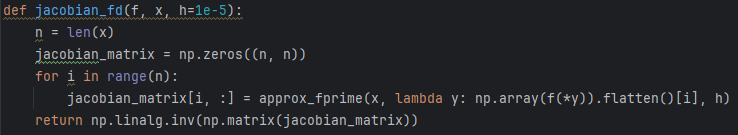
\includegraphics[width=0.75\linewidth]{jacobian.png}
            \label{fig:enter-label}
        \end{figure}
    \item \textbf{Función $f(*x)$}: Método que toma las funciones ingresadas por consolas a funciones para usar en el programa.
        \begin{figure}[H]
            \centering
            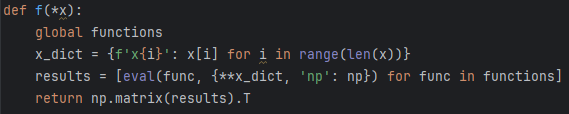
\includegraphics[width=0.75\linewidth]{f(x).png}
            \label{fig:enter-label}
        \end{figure}
    \item \textbf{Función \textit{broyden}}: Función que desarrolla el método de Broyden.
        \begin{figure}[H]
            \centering
            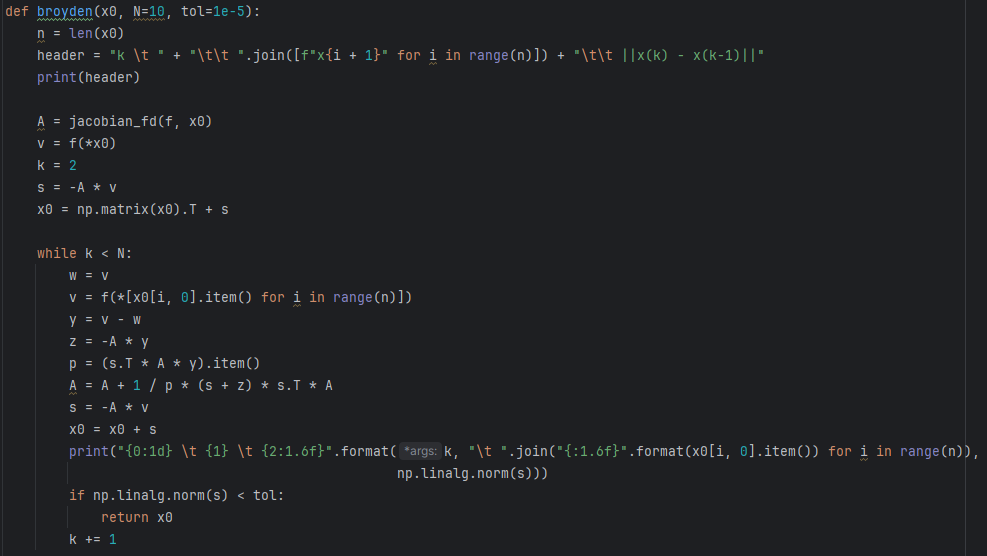
\includegraphics[width=0.75\linewidth]{broyden.png}
            \label{fig:enter-label}
        \end{figure}
    \item \textbf{Interfaz}: Ingreso de información necesaria para el desarrollo del método
        \begin{figure}[H]
            \centering
            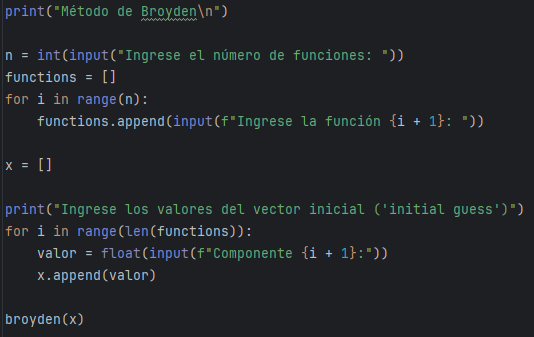
\includegraphics[width=0.75\linewidth]{interfaz.png}
            \label{fig:enter-label}
        \end{figure}
\end{itemize}

\subsection{Caso de Prueba 1}
\begin{itemize}
    \item Número de funciones: 2
    \item f1: x0**2 - x1 - 1
    \item f2: x0 - x1**2 + 1
    \item Vector inicial:
        \begin{itemize}
            \item componente 1: 1.5
            \item componente 2: 2.0
        \end{itemize}
    \item \textbf{Entrada:}
        \begin{figure}[H]
            \centering
            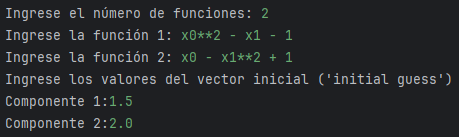
\includegraphics[width=0.75\linewidth]{entrada1.png}
            \label{fig:enter-label}
        \end{figure}
    \item \textbf{Salida:}
        \begin{figure}[H]
            \centering
            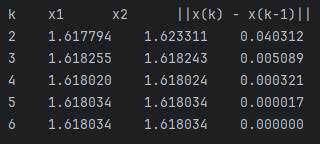
\includegraphics[width=0.75\linewidth]{salida1.png}
            \label{fig:enter-label}
        \end{figure}
\end{itemize}

\subsection{Caso de Prueba 2}
\begin{itemize}
    \item Número de funciones: 3
    \item f1: 3*x0 - np.cos(x0*x2) - 0.5
    \item f2: x0**2 - 81*(x1+0.1)**2 + np.sin(x2) + 1.06
    \item f3: np.exp(-x0*x1) + 20*x2 + (10*np.pi - 3)/3
    \item Vector inicial:
        \begin{itemize}
            \item componente 1: 0.1
            \item componente 2: 0.1
            \item componente 3: -0.1
        \end{itemize}
    \item \textbf{Entrada:}
        \begin{figure}[H]
            \centering
            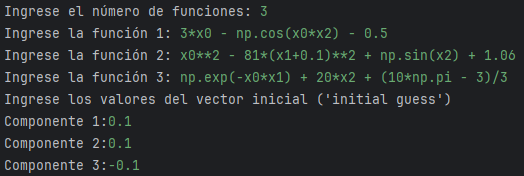
\includegraphics[width=0.75\linewidth]{entrada2.png}
            \label{fig:enter-label}
        \end{figure}
    \item \textbf{Salida:}
        \begin{figure}[H]
            \centering
            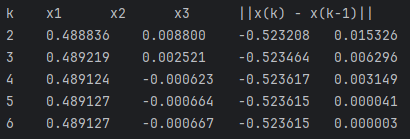
\includegraphics[width=0.75\linewidth]{salida2.png}
            \label{fig:enter-label}
        \end{figure}
\end{itemize}

\section{Conclusiones}

En síntesis, el método de Broyden se presenta como una herramienta eficaz para resolver sistemas de ecuaciones no lineales, con una convergencia de orden cuadrático. Únicamente se requiere evaluar el Jacobiano una vez o aproximarlo mediante diferencias finitas. Además, se aprovecha el uso de los valores previos de $X$ y $F$ para actualizar la inversa del Jacobiano, sin necesidad de invertir una matriz después de la primera iteración, reduciendo la cantidad de cálculos aritméticos considerablemente. Cabe mencionar que existen diversas versiones del método de Broyden, de las cuales se puede escoger aquella que nos convenga más, para efectos de seguimiento de las iteraciones o convergencia, decidiendo también si dicha versión hace valer la pena el perder velocidad de convergencia con respecto a Newton. Un método sin duda alguna útil que ofrece un equilibrio entre eficiencia computacional y convergencia, aunque en su camino sacrifica la convergencia cuadrática del mismo.

\section{ Apéndice: Método de Continuación}
La convergencia en el método de Newton (y de la secante) no siempre está garantizada. En la práctica es difícil encontrar un buen punto inicial que lleve a la convergencia de las iteraciones.

Dados $f(x)$ y $g(x)$ donde el cero $r$ para $f(x)=0$ es difícil de resolver, mientras que $g(x)=0$ es conocido, digamos $g(u)=0$, construimos una nueva función:

\begin{equation*}
    \Phi(x; s) = s f(x) + (1 - s) g(x), \quad 0 < s < 1
\end{equation*}

Si $s = 0$ tenemos $\Phi(x;0) = g(x)$, y si $s = 1$ tenemos $\Phi(x;1) = f(x)$.
Como $s$ oscila entre $0$ y $1$, el $0$ de $\Phi(x;s)$ va a moverse desde $u$ hasta $r$ de modo continuo.
Por lo tanto, tomaremos pasos pequeños, empezando desde la raíz de $g(x)$ y continuamente acercándonos a la raíz para $f(x)$.
Específicamente sea $N$ el número de pasos, y sea:

\begin{equation*}
    \Delta s = \frac{1}{N}, \quad s k = k \Delta s, \quad k = 1, 2, \ldots, N
\end{equation*}

Sea $r_0 = u$.
Para $k = 1, 2, \ldots, N$ resolvemos $\Phi(x;s_k) = 0$ con el método de newton, usando $r_{k-1}$ como el punto inicial.
Si $s$ es suficientemente pequeño, entonces $r_{k-1}$ está suficientemente cerca de $rx$ y el método de Newton converge rápidamente.
La raíz final $r_N$ será la raíz de $f(x)$.

\newpage
\citationstyle{dcu}
\addcontentsline{toc}{section}{\numberline{11} Referencias}
\bibliographystyle{plain}
\begin{thebibliography}{99}
    \harvarditem{Broyden}{$1965$}{BR65} 
	Broyden, C. G. ($1965$). A Class of Methods for Solving Nonlinear Simultaneous Equations. \textit{Mathematics of Computation}, $19(92)$, $577-593$. https://doi.org/10.2307/2003941
    \harvarditem{Muto}{MUNE} 
	MMuto, V. CAPITULO XXIII. METODOS CUASI-NEWTON. \textit{Métodos Cuasi-Newton}, $307-311$.
    \harvarditem{Moré & Trangenstein}{$1976$}{MT76} 
	Moré, J. J., \& Trangenstein, J. A. ($1976$). On the Global Convergence of Broyden’s Method. \textit{Mathematics of Computation}, $30(135)$, $523-540$. https://doi.org/10.2307/2005323
    \harvarditem{Dennis}{$1971$}{DE71} 
	Dennis, J. E. ($1971$). On the Convergence of Broyden’s Method for Nonlinear Systems of Equations. \textit{Mathematics of Computation}, $25(115)$, $559-567$. https://doi.org/10.2307/2005218
    \harvarditem{Lambers}{$2012$}{LA12} 
	Lambers, J. ($2012$). Broyden’s Method. Lecture 11 Notes \textit{Summer Session 2011-12}, $MAT 419/519$, $1-5$. https://www.math.usm.edu/lambers/mat419/lecture11.pdf
    \harvarditem{Gay}{$1979$}{GA79} 
	Gay, D. M. ($1979$). Some Convergence Properties of Broyden’s Method. \textit{SIAM Journal on Numerical Analysis}, $16(4)$, $623-630$. http://www.jstor.org/stable/2156533
    \harvarditem{Dennis}{$1971$}{DE71} 
	Martínez, J. M. ($1978$). On the order of convergence of Broyden-Gay-Schnabel's method. \textit{Commentationes Mathematicae Universitatis Carolinae}, $19(1978)$, $107-118$. http://dml.cz/dmlcz/105837
\end{thebibliography}

\end{document}
